\documentclass[border=10pt]{standalone}
\usepackage{tikz}
\usepackage{graphicx}

\begin{document}
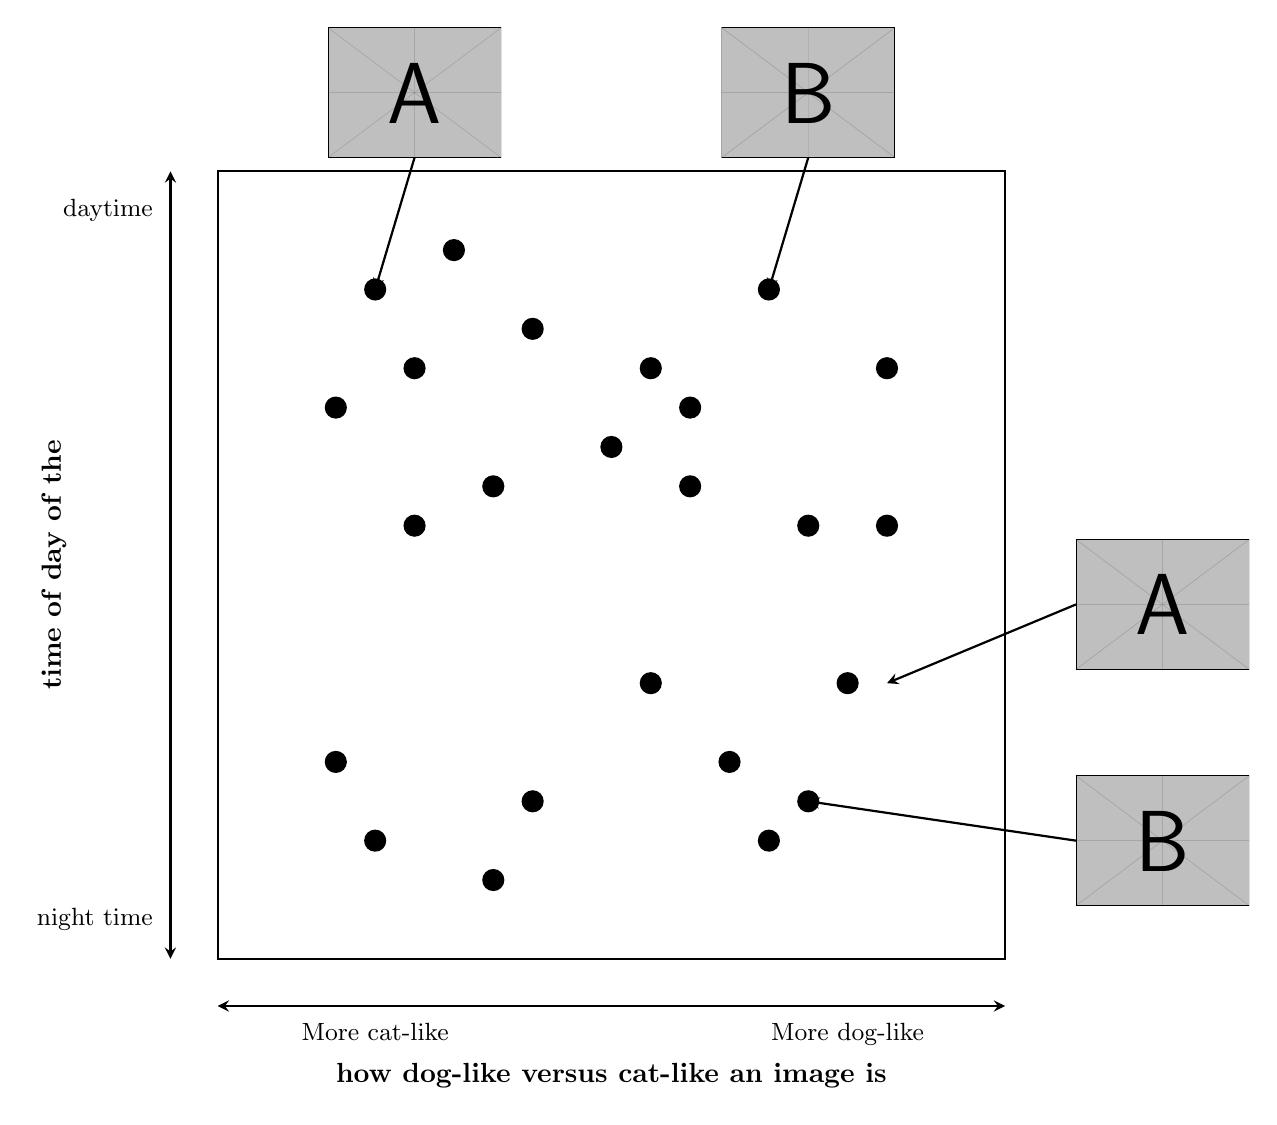
\begin{tikzpicture}[
    thumbnail/.style={inner sep=0pt, outer sep=0pt},
    arrowstyle/.style={->, thick, >=stealth},
]

% === CONFIGURATION ===
% Replace these with your own image paths:
\def\imgCatDay{example-image-a}      % top-left thumbnail (cat, daytime)
\def\imgDogDay{example-image-b}      % top-right thumbnail (dog, daytime)
\def\imgCatNight{example-image-a}     % bottom-right thumbnail #1 (cat, nighttime)
\def\imgDogNight{example-image-b}     % bottom-right thumbnail #2 (dog, nighttime)
\def\thumbsize{2.2cm}                 % thumbnail width

% === TITLE ===
\node[font=\Large\bfseries, anchor=south] at (5, 11.5)
    {};

% === MAIN BOX ===
\draw[thick] (0,0) rectangle (10,10);

% === AXES ===
% Y-axis: time of day
\draw[<->, thick, >=stealth] (-0.6, 0) -- (-0.6, 10);
\node[rotate=90, anchor=south, font=\bfseries, align=center] at (-1.8, 5)
    {time of day of the};
\node[anchor=east, font=\small] at (-0.7, 9.5) {daytime};
\node[anchor=east, font=\small] at (-0.7, 0.5) {night time};

% X-axis: cat-like vs dog-like
\draw[<->, thick, >=stealth] (0, -0.6) -- (10, -0.6);
\node[font=\bfseries, anchor=north] at (5, -1.2)
    {how dog-like versus cat-like an image is};
\node[anchor=north, font=\small] at (2, -0.7) {More cat-like};
\node[anchor=north, font=\small] at (8, -0.7) {More dog-like};

% === SCATTER POINTS ===
% Daytime cluster (upper region, mixed cat/dog)
\foreach \px/\py in {
    2.0/8.5,  3.0/9.0,
    1.5/7.0,  2.5/7.5,
    4.0/8.0,  5.5/7.5,
    6.0/7.0,  7.0/8.5,
    8.5/7.5,
    2.5/5.5,  3.5/6.0,
    5.0/6.5,  6.0/6.0,
    7.5/5.5,  8.5/5.5,
    % Nighttime cluster (lower region)
    1.5/2.5,  2.0/1.5,
    3.5/1.0,  4.0/2.0,
    6.5/2.5,  7.0/1.5,  7.5/2.0,
    5.5/3.5,  8.0/3.5
}{
    \fill (\px, \py) circle (4pt);
}

% === THUMBNAIL IMAGES ===
% Top-left: Cat + Daytime
\node[thumbnail] (catday) at (2.5, 11.0)
    {\includegraphics[width=\thumbsize]{\imgCatDay}};
\draw[arrowstyle] (catday.south) -- (2.0, 8.5);

% Top-right: Dog + Daytime
\node[thumbnail] (dogday) at (7.5, 11.0)
    {\includegraphics[width=\thumbsize]{\imgDogDay}};
\draw[arrowstyle] (dogday.south) -- (7.0, 8.5);

% Right side: Cat + Nighttime
\node[thumbnail] (catnight) at (12.0, 4.5)
    {\includegraphics[width=\thumbsize]{\imgCatNight}};
\draw[arrowstyle] (catnight.west) -- (8.5, 3.5);

% Right side: Dog + Nighttime
\node[thumbnail] (dognight) at (12.0, 1.5)
    {\includegraphics[width=\thumbsize]{\imgDogNight}};
\draw[arrowstyle] (dognight.west) -- (7.5, 2.0);

\end{tikzpicture}
\end{document}